\section{Linux Common Analysis \& Observability Tools}

\subsection{Pseudo Filesystems}

\begin{frame}
  \frametitle{Pseudo Filesystems}
  \begin{itemize}
    \item Some virtual filesystems are exposed by the kernel and provide a lot
          of information on the system.
    \item {\em procfs} contains information about processes and system
          information.
    \begin{itemize}
      \item Mounted on \code{/proc}
      \item Often parsed by tools to display raw data in a more user-friendly
            way.
    \end{itemize}
    \item {\em sysfs} provides informations about hardware/logical devices,
          association between devices and drivers.
    \begin{itemize}
      \item Mounted on \code{/sys}
    \end{itemize}
    \item {\em debugfs} exposes information related to debug.
    \begin{itemize}
      \item Typically mounted on \code{/sys/kernel/debug/}
      \item \code{mount -t debugfs none /sys/kernel/debug}
    \end{itemize}
  \end{itemize}
\end{frame}

\begin{frame}
  \frametitle{procfs}
  \begin{itemize}
    \item {\em procfs} exposes information about processes and system
          (\manpage{proc}{5}).
    \begin{itemize}
      \item \code{/proc/cpuinfo} CPU information.
      \item \code{/proc/meminfo} memory information (used, free, total, etc).
      \item \code{/proc/sys/} contains system parameters that can be tuned. The
            list of parameters that can be modified is available at
            \kdochtml{admin-guide/sysctl/index}
      \item \code{/proc/interrupts}: interrupt count per CPU for each interrupt
      in use
      \begin {itemize}
        \item We also have one entry per interrupt in \code{/proc/irq} for
        specific configuration/status for each interrupt line
      \end {itemize}
      \item \code{/proc/<pid>/} process related information
      \begin{itemize}
        \item\code{/proc/<pid>/status} process basic information
        \item \code{/proc/<pid>/maps} process memory mappings
        \item \code{/proc/<pid>/fd} file descriptors of the process
        \item \code{/proc/<pid>/task} descriptors of threads belonging
          to the process
      \end{itemize}
      \item \code{/proc/self/} will refer to the process used to access the file
    \end{itemize}
    \item A list of all available {\em procfs} file and their content is
          described at \kdochtml{filesystems/proc} and \manpage{proc}{5}
  \end{itemize}
\end{frame}

\begin{frame}
  \frametitle{sysfs}
  \begin{itemize}
    \item {\em sysfs} filesystem exposes information about various kernel
          subsystems, hardware devices and association with drivers
          (\manpage{sysfs}{5}).
    \item This allows to find the link between drivers and devices through a
          file hierarchy representing the kernel internal tree of devices.
    \item \code{/sys/kernel} contains interesting files for kernel debugging:
    \begin{itemize}
      \item \code{irq} with information about interrupts (mapping, count, etc).
      \item \code{tracing} for tracing control.
    \end{itemize}
    \item \kdochtml{admin-guide/abi-stable}
  \end{itemize}
\end{frame}

\begin{frame}
  \frametitle{debugfs}
  \begin{itemize}
    \item {\em debugfs} is a simple RAM-based filesystem which exposes debugging
          information.
    \item Used by some subsystems ({\em clk}, {\em block}, {\em dma}, {\em gpio},
          etc) to expose debugging information related to the internals.
    \item Usually mounted on \code{/sys/kernel/debug}
    \begin{itemize}
      \item Dynamic debug features exposed through
      \code{/sys/kernel/debug/dynamic_debug} (also exposed in \code{proc})
      \item Clock tree exposed through \code{/sys/kernel/debug/clk/clk_summary}.
    \end{itemize}
  \end{itemize}
\end{frame}

\subsection{ELF file analysis}

\begin{frame}
  \frametitle{ELF files}
  \begin{columns}
    \column{0.75\textwidth}
           {\bf E}xecutable and {\bf L}inkable {\bf F}ormat
      \begin{itemize}
        \item File starting with a header which holds binary structures
              defining the file
        \item Collection of segments and sections that contain data
        \begin{itemize}
          \item \code{.text} section: Code
          \item \code{.data} section: Data
          \item \code{.rodata} section: Read-only Data
          \item \code{.debug_info} section: Contains debugging information
        \end{itemize}
        \item Sections are part of a segment which can be loadable in memory
        \item Same format for all architectures supported by the kernel and also
              \code{vmlinux} format
        \begin{itemize}
          \item Also used by a lot of other operating systems as the standard
                executable file format
        \end{itemize}
      \end{itemize}
    \column{0.25\textwidth}
      \vspace{0.5cm}
      %% Source: https://commons.wikimedia.org/wiki/File:Elf-layout--en.svg
      \includegraphics[height=0.5\textheight]{slides/debugging-linux-application-stack/elf_layout.pdf}
  \end{columns}
\end{frame}

\begin{frame}[fragile]
  \frametitle{binutils for ELF analysis}
  \begin{itemize}
    \item The binutils are used to deal with binary files, either object files
          or executables.
    \begin{itemize}
      \item Includes \code{ld}, \code{as} and other useful tools.
    \end{itemize}
    \item {\em readelf} displays information about ELF files (header, section,
          segments, etc).
    \item {\em objdump} allows to display information and disassemble ELF
          files.
    \item {\em objcopy} can convert ELF files or extract/translate some
          parts of it.
    \item {\em nm} displays the list of symbols embedded in ELF files.
    \item {\em addr2line} finds the source code line/file pair from an address using
          an ELF file with debug information
  \end{itemize}
\end{frame}

\begin{frame}[fragile]
  \frametitle{binutils example (1/2)}
  \begin{itemize}
    \item Finding the address of \code{ksys_read()} kernel function using {\em nm}:
    \begin{block}{}
      \begin{minted}[fontsize=\footnotesize]{console}
$ nm vmlinux | grep ksys_read
c02c7040 T ksys_read
      \end{minted}
    \end{block}

    \item Using {\em addr2line} to match a kernel OOPS address or a symbol name
      with source code:
    \begin{block}{}
      \begin{minted}[fontsize=\footnotesize]{console}
$ addr2line -s -f -e vmlinux ffffffff8145a8b0
queue_wc_show
blk-sysfs.c:516
      \end{minted}
% The following is supported only by recent versions of addr2line, not yet on Ubuntu 22.04
% TODO add it back later, when switching to Ubuntu 24.04?
%$ addr2line -e vmlinux printk+0x10
%/home/training/debugging-labs/buildroot/output/build/linux-5.13/kernel/printk/printk.c:2211
    \end{block}
  \end{itemize}
\end{frame}

\begin{frame}[fragile]
  \frametitle{binutils example (2/2)}
  \begin{itemize}
    \item Display an elf header with {\em readelf}:
    \begin{block}{}
      \begin{minted}[fontsize=\footnotesize]{console}
$ readelf -h binary
ELF Header:
Magic:   7f 45 4c 46 02 01 01 00 00 00 00 00 00 00 00 00
Class:                             ELF64
Data:                              2's complement, little endian
Version:                           1 (current)
OS/ABI:                            UNIX - System V
ABI Version:                       0
Type:                              DYN (Position-Independent Executable file)
Machine:                           Advanced Micro Devices X86-64
...
      \end{minted}
    \end{block}

    \item Convert an elf file to a flat binary file using {\em objcopy}:
    \begin{block}{}
      \begin{minted}[fontsize=\footnotesize]{console}
$ objcopy -O binary file.elf file.bin
      \end{minted}
    \end{block}
  \end{itemize}
\end{frame}


\begin{frame}[fragile]
  \frametitle{{\em ldd}}
  \begin{itemize}
    \item In order to display the shared libraries used by an ELF binary, one
          can use {\em ldd} (Generally packaged with C library. See \manpage{ldd}{1}).
    \item {\em ldd} will list all the libraries that were used at link time.
    \begin{itemize}
      \item Libraries that are loaded at runtime using \code{dlopen()} are not
            displayed.
    \end{itemize}
  \end{itemize}
  \begin{block}{}
    \begin{minted}[fontsize=\footnotesize]{console}
$ ldd /usr/bin/bash
linux-vdso.so.1 (0x00007ffdf3fc6000)
libreadline.so.8 => /usr/lib/libreadline.so.8 (0x00007fa2d2aef000)
libc.so.6 => /usr/lib/libc.so.6 (0x00007fa2d2905000)
libncursesw.so.6 => /usr/lib/libncursesw.so.6 (0x00007fa2d288e000)
/lib64/ld-linux-x86-64.so.2 => /usr/lib64/ld-linux-x86-64.so.2 (0x00007fa2d2c88000)
    \end{minted}
  \end{block}
\end{frame}

\subsection{Monitoring tools}

\begin{frame}
  \frametitle{Monitoring Tools}
  \begin{itemize}
    \item Lots of monitoring tools on Linux to allow monitoring various part of
          the system.
    \item Most of the time, these are CLI interactive programs.
    \begin{itemize}
        \item Processes with {\em ps}, {\em top}, {\em htop}, etc
        \item Memory with {\em free}, {\em vmstat}
        \item Networking
    \end{itemize}
    \item Almost all these tools relies on the {\em sysfs} or {\em procfs}
          filesystem to obtain the processes, memory and system information but
          will display them in a more human readable way.
    \begin{itemize}
      \item Networking tools uses a netlink interface with the networking
            subsystem of the kernel.
    \end{itemize}
  \end{itemize}
\end{frame}

\subsection{Process and CPU monitoring tools}

\begin{frame}[fragile]
  \frametitle{Processes with {\em ps}}
  \begin{itemize}
    \item The {\em ps} command allows to display a snapshot of active processes and
          their associated information (\manpage{ps}{1})
    \begin{itemize}
      \item Lists both user processes and kernel threads.
      \item Displays PID, CPU usage, memory usage, uptime, etc.
    \end{itemize}
    \begin{itemize}
      \item Uses {\em /proc/<pid>/} directory to obtain process information.
      \item Always present on almost all embedded platforms (provided by
            {\em Busybox}).
    \end{itemize}
    \item By default, displays only the current user/current tty processes.
    \item Useful for scripting and parsing since its output is static.
  \end{itemize}
\end{frame}

\begin{frame}[fragile]
  \frametitle{{\em ps} example}
  \begin{itemize}
  \frametitle{Processes with {\em ps}}
    \item Display all processes in a friendly way:
  \end{itemize}
  \begin{block}{}
    \begin{minted}[fontsize=\footnotesize]{console}
$ ps aux
USER         PID %CPU %MEM    VSZ   RSS TTY      STAT START   TIME COMMAND
root           1  0.0  0.0 168864 12800 ?        Ss   09:08   0:00 /sbin/init
root           2  0.0  0.0      0     0 ?        S    09:08   0:00 [kthreadd]
root           3  0.0  0.0      0     0 ?        I<   09:08   0:00 [rcu_gp]
root           4  0.0  0.0      0     0 ?        I<   09:08   0:00 [rcu_par_gp]
root           5  0.0  0.0      0     0 ?        I<   09:08   0:00 [netns]
...
root         914  0.0  0.0 396216 16220 ?        Ssl  09:08   0:04 /usr/libexec/udisks2/udisksd
avahi        929  0.0  0.0   8728   412 ?        S    09:08   0:00 avahi-daemon: chroot helper
root         956  0.0  0.1 260304 19024 ?        Ssl  09:08   0:02 /usr/sbin/NetworkManager --no-daemon
root         960  0.0  0.0  17040  5704 ?        Ss   09:08   0:00 /sbin/wpa_supplicant -u -s -O /run/wpa_suppli
root         962  0.0  0.0 317644 11896 ?        Ssl  09:08   0:00 /usr/sbin/ModemManager
vnstat       987  0.0  0.0   5516  3696 ?        Ss   09:08   0:00 /usr/sbin/vnstatd -n
    \end{minted}
  \end{block}
\end{frame}

\begin{frame}[fragile]
  \frametitle{Processes with {\em top}}
  \begin{itemize}
    \item {\em top} command output information similar to {\em ps} but dynamic
          and interactive (\manpage {top}{1}).
    \begin{itemize}
      \item Also almost always present on embedded platforms (provided by
            {\em Busybox})
    \end{itemize}
  \end{itemize}
  \begin{block}{}
    \begin{minted}[fontsize=\footnotesize]{console}
$ top
top - 18:38:11 up  9:29,  1 user,  load average: 2.84, 2.74, 2.02
Tasks: 371 total,   1 running, 370 sleeping,   0 stopped,   0 zombie
%Cpu(s):  5.8 us,  2.1 sy,  0.0 ni, 77.4 id, 14.7 wa,  0.0 hi,  0.0 si,  0.0 st
MiB Mem :  15947.6 total,   1476.9 free,   7685.7 used,   6784.9 buff/cache
MiB Swap:  15259.0 total,  15238.7 free,     20.2 used.   7742.3 avail Mem

    PID USER      PR  NI    VIRT    RES    SHR S  %CPU  %MEM     TIME+ COMMAND
   2988 cleger    20   0 5184816   1.2g 430244 S  26.7   7.9  60:24.27 firefox-esr
   4326 cleger    20   0   16.4g 208104  81504 S  26.7   1.3   9:27.33 code
    909 root     -51   0       0      0      0 S  13.3   0.0  15:12.15 irq/104-nvidia
  41704 cleger    20   0   38.4g 373744 116984 S  13.3   2.3  13:25.76 code
  91926 cleger    20   0 2514784 145360  95144 S  13.3   0.9   1:29.85 Web Content
    \end{minted}
  \end{block}
\end{frame}

\begin{frame}[fragile]
  \frametitle{mpstat}
  \begin{itemize}
    \item {\em mpstat} displays Multiprocessor statistics (\manpage{mpstat}{1}).
    \item Useful to detect unbalance CPU workloads, bad IRQ affinity, etc.
  \end{itemize}
  \begin{block}{}
    \begin{minted}[fontsize=\scriptsize]{console}
$ mpstat -P ALL
Linux 6.0.0-1-amd64 (fixe)      19/10/2022      _x86_64_        (4 CPU)

17:02:50     CPU    %usr   %nice    %sys %iowait    %irq   %soft  %steal  %guest  %gnice   %idle
17:02:50     all    6,77    0,00    2,09   11,67    0,00    0,06    0,00    0,00    0,00   79,40
17:02:50       0    6,88    0,00    1,93    8,22    0,00    0,13    0,00    0,00    0,00   82,84
17:02:50       1    4,91    0,00    1,50    8,91    0,00    0,03    0,00    0,00    0,00   84,64
17:02:50       2    6,96    0,00    1,74    7,23    0,00    0,01    0,00    0,00    0,00   84,06
17:02:50       3    9,32    0,00    2,80   54,67    0,00    0,00    0,00    0,00    0,00   33,20
17:02:50       4    5,40    0,00    1,29    4,92    0,00    0,00    0,00    0,00    0,00   88,40
    \end{minted}
  \end{block}
\end{frame}

\subsection{Memory monitoring tools}

\begin{frame}[fragile]
  \frametitle{{\em free}}
  \begin{itemize}
    \item {\em free} is a simple program that displays the amount of free and
          used memory in the system (\manpage{free}{1}).
    \begin{itemize}
      \item Useful to check if the system suffers from memory exhaustion
      \item Uses \code{/proc/meminfo} to obtain memory information.
    \end{itemize}
  \end{itemize}
  \begin{block}{}
    \begin{minted}[fontsize=\footnotesize]{console}
$ free -h
               total        used        free      shared  buff/cache   available
Mem:            15Gi       7.5Gi       1.4Gi       192Mi       6.6Gi       7.5Gi
Swap:           14Gi        20Mi        14Gi
    \end{minted}
  \end{block}
  \begin{itemize}
    \item {\em A small \code{free} value does not mean that your system suffers
    from memory depletion! Linux considers any unused memory as "wasted" so
    it uses it for buffers and caches to optimize performance. See also
    \code{drop_caches} from \manpage{proc}{5} to observe buffers/cache
    impact on free/available memory}
  \end{itemize}
\end{frame}

\begin{frame}[fragile]
  \frametitle{vmstat}
  \begin{itemize}
    \item {\em vmstat} displays information about system virtual memory usage
    \item Can also display stats from processes, memory, paging, block IO,
          traps, disks and cpu activity (\manpage{vmstat}{8}).
    \item Can be used to gather data at periodic interval using \code{vmstat <interval> <number>}
  \end{itemize}
  \begin{block}{}
    \begin{minted}[fontsize=\footnotesize]{console}
$ vmstat 1 6
procs -----------memory----------   ---swap--  -----io---- -system-- ------cpu-----
r  b   swpd   free   buff  cache     si   so    bi    bo    in   cs  us sy id wa st
3  0 253440 1237236 194936 9286980    3    6   186   540    134  157  3  5 82 10  0
    \end{minted}
  \end{block}
  \begin{itemize}
    \item {\em Note: vmstat consider a kernel block to be 1024 bytes}
  \end{itemize}
\end{frame}

\begin{frame}[fragile]
  \frametitle{pmap}
  \begin{itemize}
    \item \code{pmap} displays process mappings more easily than
          accessing \code{/proc/<pid>/maps} (\manpage{pmap}{1}).
  \end{itemize}
  \begin{block}{}
    \begin{minted}[fontsize=\tiny]{console}
# pmap 2002
2002:   /usr/bin/dbus-daemon --session --address=systemd: --nofork --nopidfile --systemd-activation --syslog-only
...
00007f3f958bb000     56K r---- libdbus-1.so.3.32.1
00007f3f958c9000    192K r-x-- libdbus-1.so.3.32.1
00007f3f958f9000     84K r---- libdbus-1.so.3.32.1
00007f3f9590e000      8K r---- libdbus-1.so.3.32.1
00007f3f95910000      4K rw--- libdbus-1.so.3.32.1
00007f3f95937000      8K rw---   [ anon ]
00007f3f95939000      8K r---- ld-linux-x86-64.so.2
00007f3f9593b000    152K r-x-- ld-linux-x86-64.so.2
00007f3f95961000     44K r---- ld-linux-x86-64.so.2
00007f3f9596c000      8K r---- ld-linux-x86-64.so.2
00007f3f9596e000      8K rw--- ld-linux-x86-64.so.2
00007ffe13857000    132K rw---   [ stack ]
00007ffe13934000     16K r----   [ anon ]
00007ffe13938000      8K r-x--   [ anon ]
 total            11088K
    \end{minted}
  \end{block}
\end{frame}

\subsection{I/O monitoring tools}

\begin{frame}[fragile]
  \frametitle{iostat}
  \begin{itemize}
    \item {\em iostat} displays information about IOs per device on the system.
    \item Useful to see if a device is overloaded by IOs.
  \end{itemize}
  \begin{block}{}
    \begin{minted}[fontsize=\footnotesize]{console}
$ iostat
Linux 5.19.0-2-amd64 (fixe)     11/10/2022      _x86_64_        (12 CPU)

avg-cpu:  %user   %nice %system %iowait  %steal   %idle
           8,43    0,00    1,52    8,77    0,00   81,28

Device      tps  kB_read/s  kB_wrtn/s  kB_dscd/s  kB_read  kB_wrtn  kB_dscd
nvme0n1   55,89    1096,88     149,33       0,00  5117334   696668        0
sda        0,03       0,92       0,00       0,00     4308        0        0
sdb      104,42     274,55    2126,64       0,00  1280853  9921488        0
    \end{minted}
  \end{block}
\end{frame}

\begin{frame}[fragile]
  \frametitle{iotop}
  \begin{itemize}
    \item {\em iotop} displays information about IOs much like {\em top} for each
          process.
    \item Useful to find applications generating too much I/O traffic.
    \begin{itemize}
    \item Needs \kconfigval{CONFIG_TASKSTATS}{y},
          \kconfigval{CONFIG_TASK_DELAY_ACCT}{y} and
          \kconfigval{CONFIG_TASK_IO_ACCOUNTING}{y} to be enabled in the
          kernel.
    \item Also needs to be enabled at runtime: \code{sysctl -w kernel.task_delayacct=1}
    \end{itemize}
  \end{itemize}
  \begin{block}{}
    \begin{minted}[fontsize=\small]{console}
# iotop
Total DISK READ:        20.61 K/s | Total DISK WRITE:        51.52 K/s
Current DISK READ:      20.61 K/s | Current DISK WRITE:      24.04 K/s
    TID  PRIO  USER     DISK READ DISK WRITE>    COMMAND
    2629 be/4 cleger     20.61 K/s   44.65 K/s firefox-esr [Cache2 I/O]
    322 be/3 root        0.00 B/s    3.43 K/s [jbd2/nvme0n1p1-8]
  39055 be/4 cleger      0.00 B/s    3.43 K/s firefox-esr [DOMCacheThread]
      1 be/4 root        0.00 B/s    0.00 B/s init
      2 be/4 root        0.00 B/s    0.00 B/s [kthreadd]
      3 be/0 root        0.00 B/s    0.00 B/s [rcu_gp]
      4 be/0 root        0.00 B/s    0.00 B/s [rcu_par_gp]
      ...
    \end{minted}
  \end{block}
\end{frame}

\setuplabframe
{System Status}
{
  Check what is running on a system and its load
  \begin{itemize}
    \item Observe processes and IOs
    \item Display memory mappings
    \item Monitor resources
  \end{itemize}
}

\subsection{Networking observability tools}

\begin{frame}{ss}
  \begin{itemize}
  \item {\em ss} shows the status of network sockets
    \begin{itemize}
    \item IPv4 and IPv6, UDP, TCP, ICMP and UNIX domain sockets
    \end{itemize}
  \item Replaces {\em netstat}, now obsolete
  \item Gets info from \code{/proc/net}
  \item Usage:\\
    \code{ss} by default shows connected sockets\\
    \code{ss -l} shows listening sockets\\
    \code{ss -a} shows both listening and connected sockets\\
    \code{ss -4/-6/-x} shows only IPv4, IPv6, or UNIX sockets\\
    \code{ss -t/-u} shows only TCP or UDP sockets\\
    \code{ss -p} shows process using each socket\\
    \code{ss -n} shows numeric addresses\\
    \code{ss -s} shows a summary of existing sockets
    \item See
      \href{https://www.man7.org/linux/man-pages/man8/ss.8.html}{the ss
        manpage} for all the options
  \end{itemize}
\end{frame}

\begin{frame}[fragile]{ss example output}
    \begin{block}{}
      \begin{minted}[fontsize=\scriptsize]{console}
# ss
Netid State  Recv-Q Send-Q                Local Address:Port            Peer Address:Port  Process
u_dgr ESTAB  0      0                                 * 304840                     * 26673
u_str ESTAB  0      0       /run/dbus/system_bus_socket 42871                      * 26100
icmp6 UNCONN 0      0                                 *:ipv6-icmp                  *:*
udp   ESTAB  0      0          192.168.10.115%wlp0s20f3:bootpc         192.168.10.88:bootps
tcp   ESTAB  0      136                      172.16.0.1:41376           172.16.11.42:ssh
tcp   ESTAB  0      273                    192.168.1.77:55494          87.98.181.233:https
tcp   ESTAB  0      0                   [2a02:...:dbdc]:38466     [2001:...:9]:imap2
...
#
      \end{minted}
    \end{block}
\end{frame}

\begin{frame}{iftop}
  \begin{itemize}
  \item {\em iftop} displays bandwidth usage on an interface by remote host
  \item Visualizes bandwidth using histograms
  \item \code{iftop -i eth0}
  \begin{center}
    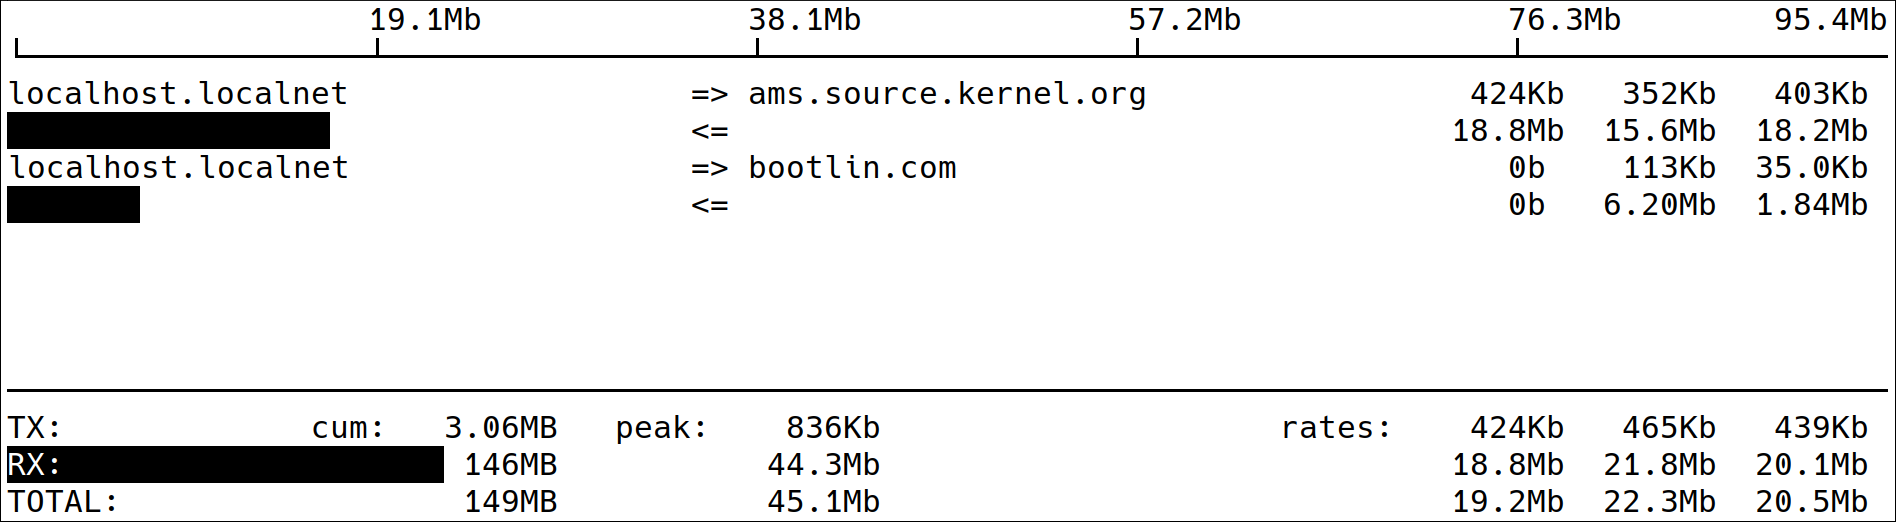
\includegraphics[width=0.9\textwidth]{slides/debugging-common-tools/iftop.png}
  \end{center}
  \item The output can be customized interactively
    \item See \href{https://linux.die.net/man/8/iftop}{the iftop manpage}
      for details
  \end{itemize}
\end{frame}

\begin{frame}{tcpdump}
  \begin{itemize}
  \item {\em tcpdump} allows to capture network traffic and decode many
    protocols
  \item \code{tcpdump -i eth0}
  \item based on the {\em libpcap} library for packet capture
  \item It can also store captured packets to a file and read them back
    \begin{itemize}
    \item In the {\em pcap} format or the newer {\em pcapng} format
    \item \code{tcpdump -i eth0 -w capture.pcap}
    \item \code{tcpdump -r capture.pcap}
    \end{itemize}
  \item A capture filter can be used to avoid capturing irrelevant packets
    \begin{itemize}
    \item \code{tcpdump -i eth0 tcp and not port 22}
    \end{itemize}
  \item \url{https://www.tcpdump.org/}
  \end{itemize}
\end{frame}

\begin{frame}[fragile]{tcpdump example output}
    \begin{block}{}
      \begin{minted}[fontsize=\scriptsize]{console}
# tcpdump -i eth0
18:41:22.913058 IP localhost.localnet.40764 > srv.localnet: 14324+ AAAA? bootlin.com. (29)
18:41:22.913797 IP srv.localnet > localhost.localnet.40764: 14324 0/1/0 (89)
18:41:22.914268 IP localhost.localnet > bootlin.com: ICMP echo request, id 3, seq 1, length 64
18:41:23.933063 IP localhost.localnet > bootlin.com: ICMP echo request, id 3, seq 2, length 64
18:41:24.957027 IP localhost.localnet > bootlin.com: ICMP echo request, id 3, seq 3, length 64
18:41:24.996415 IP bootlin.com > localhost.localnet: ICMP echo reply, id 3, seq 3, length 64
^C
# tcpdump -i eth0 tcp and not port 22
... IP B.https > A.38910: Flags [.], ack 469, win 501, options [...], length 0
... IP B.https > A.38910: Flags [P.], seq 2602:2857, ack 469, win 501, options [...], length 255
... IP A.38910 > B.https: Flags [.], ack 2857, win 501, options [...], length 0
... IP A.38910 > B.https: Flags [P.], seq 469:621, ack 2857, win 501, options [...], length 152
... IP B.https > A.38910: Flags [.], ack 621, win 501, options [...], length 0
... IP B.https > A.38910: Flags [P.], seq 2857:3825, ack 621, win 501, options [...], length 968
... IP A.38910 > B.https: Flags [P.], seq 621:779, ack 3825, win 501, options [...], length 158
^C
#
      \end{minted}
    \end{block}
\end{frame}
